% THIS IS SIGPROC-SP.TEX - VERSION 3.1
% WORKS WITH V3.2SP OF ACM_PROC_ARTICLE-SP.CLS
% APRIL 2009
%
% It is an example file showing how to use the 'acm_proc_article-sp.cls' V3.2SP
% LaTeX2e document class file for Conference Proceedings submissions.
% ----------------------------------------------------------------------------------------------------------------
% This .tex file (and associated .cls V3.2SP) *DOES NOT* produce:
%       1) The Permission Statement
%       2) The Conference (location) Info information
%       3) The Copyright Line with ACM data
%       4) Page numbering
% ---------------------------------------------------------------------------------------------------------------
% It is an example which *does* use the .bib file (from which the .bbl file
% is produced).
% REMEMBER HOWEVER: After having produced the .bbl file,
% and prior to final submission,
% you need to 'insert'  your .bbl file into your source .tex file so as to provide
% ONE 'self-contained' source file.
%
% Questions regarding SIGS should be sent to
% Adrienne Griscti ---> griscti@acm.org
%
% Questions/suggestions regarding the guidelines, .tex and .cls files, etc. to
% Gerald Murray ---> murray@hq.acm.org
%
% For tracking purposes - this is V3.1SP - APRIL 2009

\documentclass{acm_proc_article-sp}

\usepackage{graphicx}
\usepackage{caption}
\usepackage{subcaption}

\begin{document}

\title{On the Ground Validation of Online Diagnosis with Twitter and Medical Records}

%
% You need the command \numberofauthors to handle the 'placement
% and alignment' of the authors beneath the title.
%
% For aesthetic reasons, we recommend 'three authors at a time'
% i.e. three 'name/affiliation blocks' be placed beneath the title.
%
% NOTE: You are NOT restricted in how many 'rows' of
% "name/affiliations" may appear. We just ask that you restrict
% the number of 'columns' to three.
%
% Because of the available 'opening page real-estate'
% we ask you to refrain from putting more than six authors
% (two rows with three columns) beneath the article title.
% More than six makes the first-page appear very cluttered indeed.
%
% Use the \alignauthor commands to handle the names
% and affiliations for an 'aesthetic maximum' of six authors.
% Add names, affiliations, addresses for
% the seventh etc. author(s) as the argument for the
% \additionalauthors command.
% These 'additional authors' will be output/set for you
% without further effort on your part as the last section in
% the body of your article BEFORE References or any Appendices.

\numberofauthors{3} %  in this sample file, there are a *total*
% of EIGHT authors. SIX appear on the 'first-page' (for formatting
% reasons) and the remaining two appear in the \additionalauthors section.
%
\author{
% You can go ahead and credit any number of authors here,
% e.g. one 'row of three' or two rows (consisting of one row of three
% and a second row of one, two or three).
%
% The command \alignauthor (no curly braces needed) should
% precede each author name, affiliation/snail-mail address and
% e-mail address. Additionally, tag each line of
% affiliation/address with \affaddr, and tag the
% e-mail address with \email.
%
% 1st. author
\alignauthor
Todd Bodnar\titlenote{Corresponding author}\\
       \affaddr{Pennsylvania State University}\\
\affaddr{Department of Biology}\\
       \affaddr{University Park, PA 16802}\\
       \email{tjb5215@psu.edu}
% 2nd. author
\alignauthor
Maybe Conrad, Maybe Vicky
% 3rd. author
\alignauthor
Marcel Salath\'e\\
       \affaddr{Pennsylvania State University}\\
\affaddr{Department of Biology}\\
       \affaddr{University Park, PA 16802}\\
       \email{salathe@psu.edu}
}

\maketitle
\begin{abstract}
This is an abstract
\end{abstract}

% A category with the (minimum) three required fields
%\category{I.6.4}{Simulation and Modeling}{Model Validation and Analysis}
\category{I.2.1}{Artificial Intelligence}{Applications and Expert Systems}[Medicine and Science]
%A category including the fourth, optional field follows...
%\category{D.2.8}{Software Engineering}{Metrics}[complexity measures, performance measures]

\terms{Experimentation, Validation}

\keywords{Twitter, Validation, Digital Epidemiology, Remote Diagnosis} % NOT required for Proceedings

\section{Introduction}
Digital epidemiology \(\to\) novel disease detection mechanisms.

Validation of this idea is important, but not done.

Pull med info of individuals professionally diagnosed with ILI and their twitter accts. Compare old methods. Suggest some new things.

\section{Related Work}

People with issues \cite{Bodnar:2013we,Butler:2013uh,Lamb:2013to} also plos paper!

Most work to this point considers finding messages in tweets (i.e. ``I'm sick'') or in keyword frequencies. 

Keyword \cite{Culotta:2010hx,Goel:2010jf}

Tweet classification \cite{Culotta:2010hx,Lamb:2013to,Salathe:2011gr}

\section{Data Collection}
\subsection{Medical Records}
\subsection{Twitter Records}
We received a total of 119 user accounts for Twitter from the survey; 15 of which were discarded because the screen names were either non-existent, banned, or private. For each of the remaining 104 accounts, we pulled their profile information, their friends and followers information, their most recent 3000 tweets, and their friends profiles and tweets. Some users did not tweet during the month that they were sick; we kept those accounts as part of the control group. We were limited to the most recent 3000 tweets by Twitter's time line query, but this only effected two accounts -- both of which posted multiple times per hour and were thrown out because we could only look back a few days.

We collected data by calling the Twitter API on the user account that we queried the longest time ago. Tweets, profile and follower information queries have separate rate limits and were collected in parallel. The 104 seed accounts collected above were given higher priority over their friends and followers. In total, we collected 37,599 tweets from the seed accounts and XX tweets from YY accounts that they either followed or were followed by.


\section{Signal Detection}
\subsection{Event Based Signals}

In this section, we consider diagnosis based on classifying an individual tweet's content as either about ILI or not. We begin by dividing the tweets into two sets: tweets that were posted the same month that a user was sick, and tweets that were posted other times. We find a total of 1609 tweets from 35 users in the first category.

First we go the route of AUTHOR and AUTHOR by defining a set of keywords that are positive signals of influenza. We chose \{flu, influenza, sick, cough, cold, medicine, fever\} as our set of keywords. Of these seven keywords, we find a significant effect in 6 of the keywords during months when the user had ILI. (See table \ref{tab:tweet_keyword_expert_results}). Additionally, we try algorithmically selecting keywords by first finding the 12,393 most common keywords in the data set.  We then rank them based off of information gain and choose the top 10,100 or 1000 keywords from the list. In both of these cases, we preprocess the data by tokenizing the text on the characters ``.,;:'"()?!'' - as well as spaces, tabs and line breaks - remove stop words\footnote{Stop words taken from Weka's stoplist version 3.7.10.}, perform Porter stemming \cite{Porter:1980dd,Willett:2006vb}  and convert the text to lower case. We then use the occurance or absence of these keywords as features for classification. We use naive bayes, random forest, J48, logistic regression and support vector machines to classify a user as being sick in a given month or not (see figure \ref{fig:roc_keyword}).

\begin{figure} [h]
\centering
\begin{subfigure}[b]{.2\textwidth}
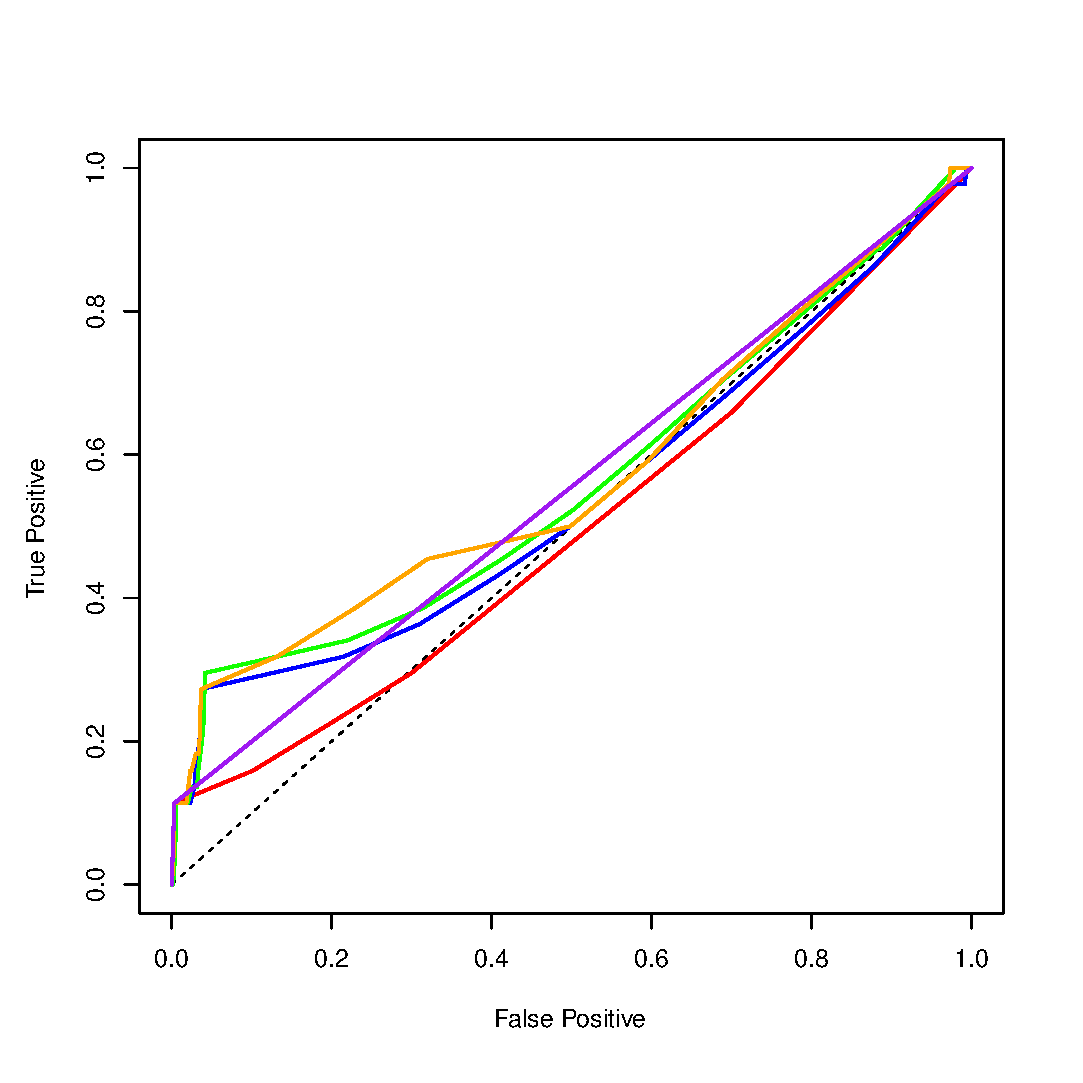
\includegraphics[width=\textwidth]{figs/key_exp_roc.eps}
\end{subfigure}
\begin{subfigure}[b]{.2\textwidth}
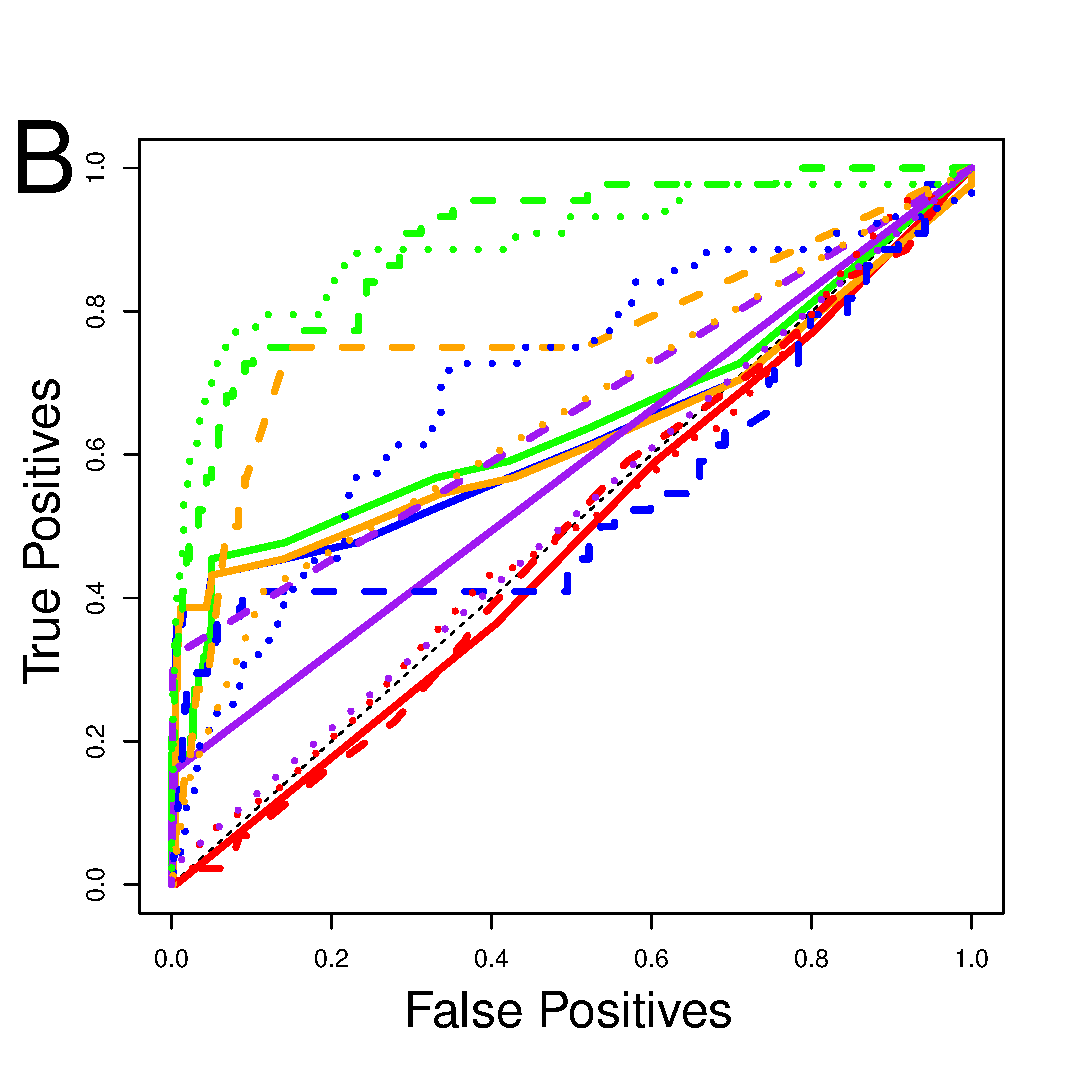
\includegraphics[width=\textwidth]{figs/key_dm_roc.eps}
\end{subfigure}
\caption{The ROC of classifiers that use hand chosen keywords (a) and algorithmically chosen keywords (b) to determine if an individual is ill. The top 10 (solid line), 100 (dashed line) and 1000 (double dashed line) were selected as the features. (COMMENT: untill I add it to figures. Green is Naive bayes, red is j48, blue is logistic, orange is random forest and purple is SVM.)}
\label{fig:roc_keyword}
\end{figure}



Additionally, we hand rate all 1609 tweets, that were posted by individuals during the time of their illness,  for information regarding the user's health. Additionally we sample a randomly selected set of 1609 tweets from times when the users did not have ILI as a control. We find 58 tweets from 17 (\(17/35 = 48.57\%\))  individuals in our study that are about the user being sick. We also find zero tweets about ILI during times when they did \textit{not} have ILI. Thus we would expect a health monitoring system based off of tweet classification to operate with at most 82.18\% accuracy. (See table \ref{tab:tweet_classified_confusion})

%flu&25&40.14& \textless 0.0001 \ \\ \hline 
influenza&1&0.00&0.8325\ \\ \hline 
sick&128&5.22& \textless 0.0001 \ \\ \hline 
cough&18&4.48&0.0094\ \\ \hline 
cold&82&1.45&0.4154\ \\ \hline 
medicin&9&11.20& \textless 0.0001 \ \\ \hline 
fever&13&26.20& \textless 0.0001 \ \\ \hline 


\begin{table}
\centering
\begin{tabular}{|c|c|c|c|} \hline
Word& Total &Odds Ratio & Significance\ \\ \hline
flu&25&40.14& \textless 0.0001 \ \\ \hline 
influenza&1&0.00&0.8325\ \\ \hline 
sick&128&5.22& \textless 0.0001 \ \\ \hline 
cough&18&4.48&0.0094\ \\ \hline 
cold&82&1.45&0.4154\ \\ \hline 
medicin&9&11.20& \textless 0.0001 \ \\ \hline 
fever&13&26.20& \textless 0.0001 \ \\ \hline 

\end{tabular}
\caption{Keyword effects.}
\label{tab:tweet_keyword_expert_results}
\end{table}

\begin{table}
\centering
\begin{tabular}{|c|c|c|} \hline
Sick&Not Sick&\ \\ \hline
1 & 2& Sick\\ \hline
3 & 4  & Not Sick\\
\hline\end{tabular}
\caption{Confusion matrix of a classifier based on keywords from a domain expert. Rows are of true values, columns are of predicted values.}
\label{tab:tweet_keyword_expert_confusion}
\end{table}

\begin{table}
\centering
\begin{tabular}{|c|c|c|} \hline
Sick&Not Sick&\ \\ \hline
1 & 2& Sick\\ \hline
3 & 4  & Not Sick\\
\hline\end{tabular}
\caption{Confusion matrix of a classifier based on keywords derived from an algorithmic aproach. Rows are of true values, columns are of predicted values.}
\label{tab:tweet_keyword_algorithm_classified_confusion}
\end{table}

\begin{table}
\centering
\begin{tabular}{|c|c|c|} \hline
Sick&Not Sick&\ \\ \hline
17 & 18 & Sick\\ \hline
0 & 66  & Not Sick\\
\hline\end{tabular}
\caption{Confusion matrix of a Tweet-Classification based diagnosis system. Rows are of true values, columns are of predicted values.}
\label{tab:tweet_classified_confusion}
\end{table}

\subsection{Frequency Based Signals}

We perform one-dimensional anomaly detection on each user's monthly tweeting rate as follows. First, we calculate the number of tweets in each month in the study period and discard any months where the user tweets less than ten times. This avoids issues caused by the user starting or stopping to use Twitter. We then calculate the z-score of the tweeting rate of the month that the user is ill by

\begin{equation}
z = \frac{|x - \bar{x}|}{\hat{s}}
\end{equation}

Where \(\bar{x}\) and \(\hat{s}\) are the estimated mean and standard deviation of the user's tweeting rate. \cite{Grubs:1969ab} We repeat this process for months when the user is not sick. We then decide that the user is sick if \(z > 1.411\) where \(1.411\) was chosen through leave one out cross validation. We find a significant difference between the z-scores for months when a user was had ILI and months when the user did not (\(p = 0.01303\), two-sample Kolmogorov-Smirnov test). Most of the time individuals are not sick (219 / 258 = 84.88\%), resulting in a highly biased sample. Thus we optimize based on the \(F_1\) score. The optimal z-score cutoff results in \(F_1= 35.0\%\). (See table \ref{tab:tweet_anomaly_confusion}.) 


%\begin{figure} %need to redo
%\centering
%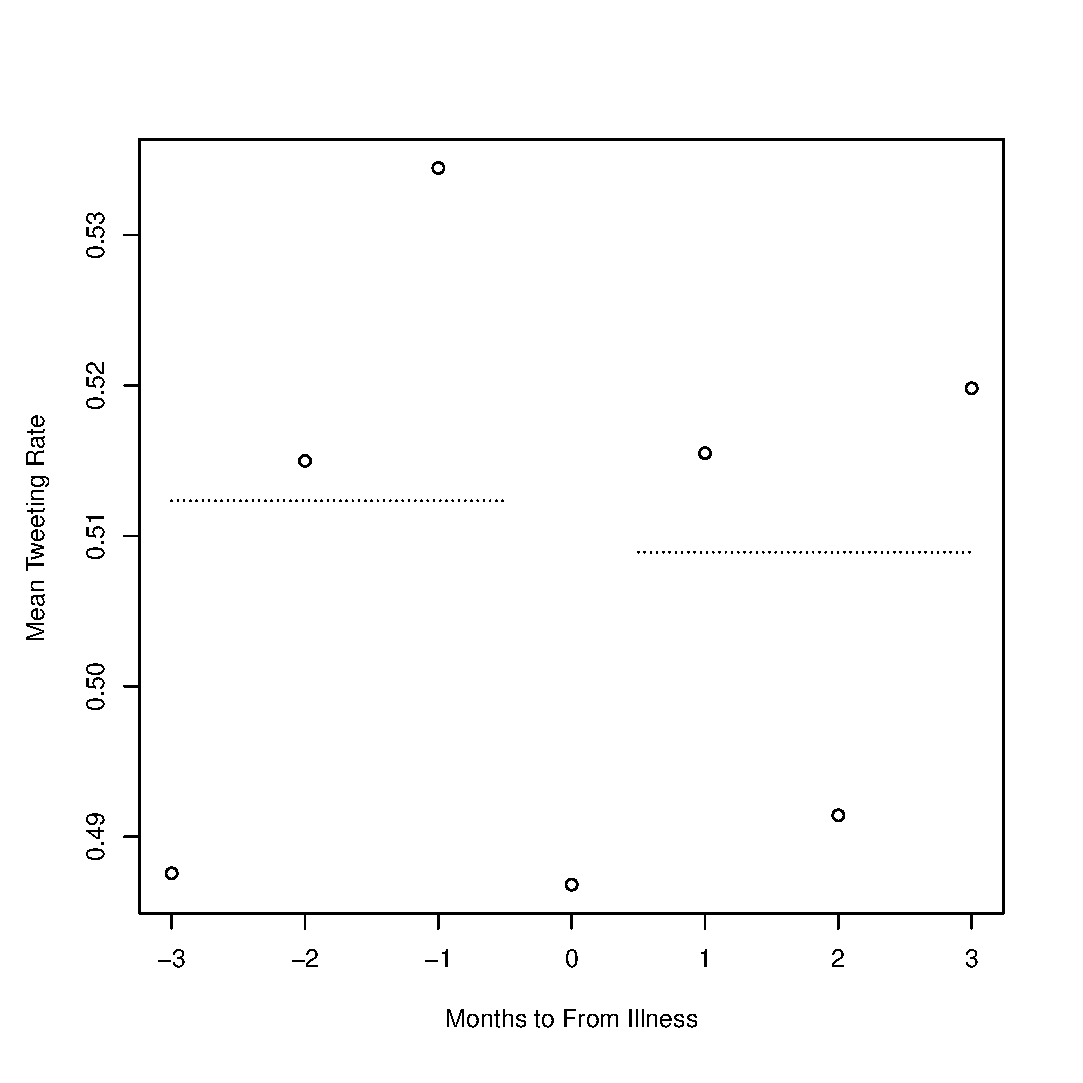
\includegraphics[width=0.5\textwidth]{figs/meanFrequencies.eps}
%\caption{The frequency of tweeting behaviour of individuals in the months before, during and after an illness. Users significantly (check) decrease their rate of tweeting during the time that they had influenza. Dashed lines indicate the mean rate for the three months before / after the illness. (Todo: check significance)}
%\label{fig:mean_freq}
%\end{figure}


\begin{table}
\centering
\begin{tabular}{|c|c|c|} \hline
Sick&Not Sick&\ \\ \hline
14 & 25 & Sick\\ \hline
27 & 192 & Not Sick\\
\hline\end{tabular}
\caption{Confusion matrix of the classifier based on anomalous tweeting rates. Rows are of true values, columns are of predicted values.}
\label{tab:tweet_anomaly_confusion}
\end{table}


\subsection{Network Based Signals}

Preliminary idea. Cascade effects causing echoes on social network. Also consider friends becoming ill around same time. Check @ tag

\section{Meta Classifier}

Combine features based off of previous signals, get something that's -- hopefully -- more accurate.


\begin{figure} [h]
\centering
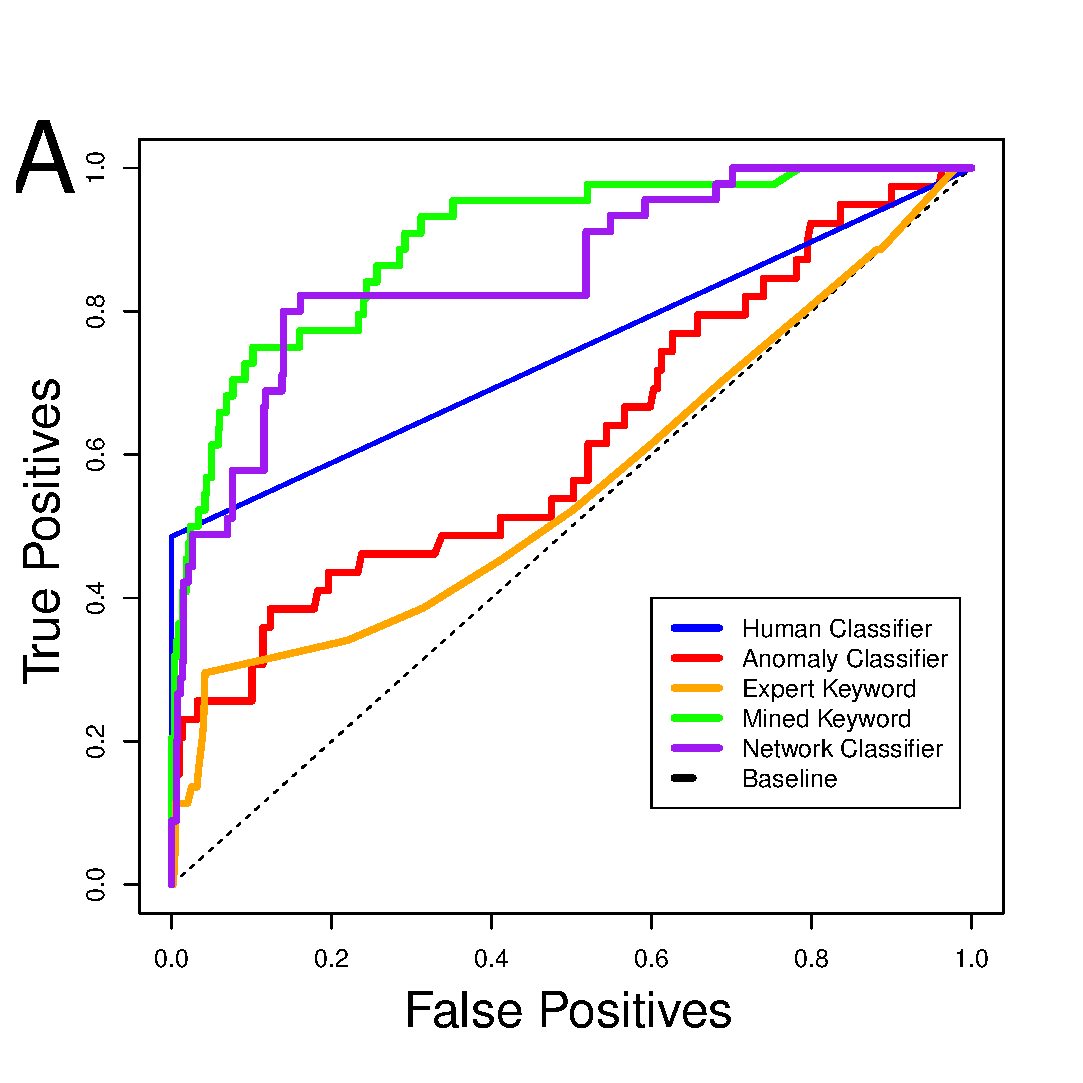
\includegraphics[width=0.4\textwidth]{figs/meta_roc.eps}
\caption{The accuracy of the previous classifiers (a) and the accuracy of various classifiers that use the previous classifier's results as features (b). }
\label{fig:roc_meta}
\end{figure}

\section{Analysis}

\section{Conclusions}

Comment on \(\sim\) 250 mill active T users \(\to\) 75 mill active US users, possibility of detecting \(\sim\) 10\% anual ILI rate, \(\sim\) half are detectable on twitter Twitter, so 12.5 mill cases as upper estimate.

%\begin{thebibliography}{1}
%\bibitem{Ford:1956vc}
%L. R. Ford and D. R. Fulkerson. \newblock{Maximal Flow through a Network}. \newblock{\em Canadian Journal of Mathematics}, 8(3):399-404, 1956.
%\end{thebibliography}



%@article{Ford:1956vc,
%author = {Ford, L R and Fulkerson, D R},
%title = {{Maximal Flow through a Network.}},
%journal = {Canadian Journal of Mathematics},
%year = {1956},
%pages = {399--404}
%}


%
% The following two commands are all you need in the
% initial runs of your .tex file to
% produce the bibliography for the citations in your paper.
\bibliographystyle{abbrv}
\bibliography{library}  % sigproc.bib is the name of the Bibliography in this case
% You must have a proper ".bib" file
%  and remember to run:
% latex bibtex latex latex
% to resolve all references
%
% ACM needs 'a single self-contained file'!
%
%APPENDICES are optional
%\balancecolumns

\balancecolumns
% That's all folks!
\end{document}
